\documentclass[10pt, onecolumn]{article}
\usepackage{tabularx}
\usepackage{tikz}
\begin{document}


\tikzset{every picture/.style={line width=0.75pt}} %set default line width to 0.75pt        

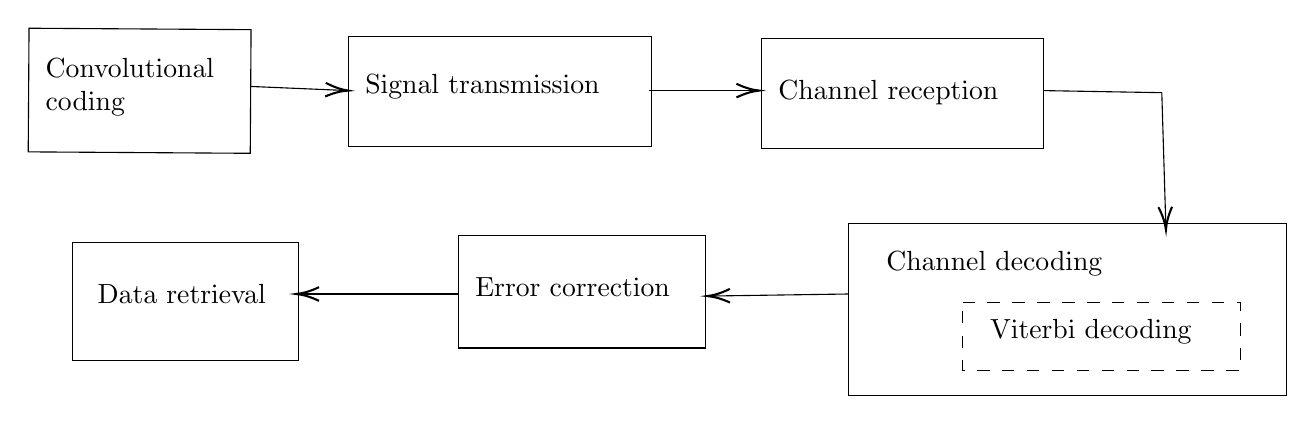
\begin{tikzpicture}[x=0.75pt,y=0.75pt,yscale=-1,xscale=1]
%uncomment if require: \path (0,300); %set diagram left start at 0, and has height of 300

%Shape: Rectangle [id:dp47147121431531436] 
\draw   (25.24,20.95) -- (132.21,21.64) -- (131.82,81.21) -- (24.85,80.52) -- cycle ;
%Shape: Rectangle [id:dp6699181989834492] 
\draw   (179,25) -- (325,25) -- (325,78) -- (179,78) -- cycle ;
%Shape: Rectangle [id:dp13625380852022662] 
\draw   (378,26) -- (514,26) -- (514,79) -- (378,79) -- cycle ;
%Shape: Rectangle [id:dp7604816059628322] 
\draw   (420,115) -- (631,115) -- (631,198) -- (420,198) -- cycle ;
%Shape: Rectangle [id:dp09128390751102777] 
\draw   (232,121) -- (351,121) -- (351,175) -- (232,175) -- cycle ;
%Shape: Rectangle [id:dp3624421410733156] 
\draw   (46,124) -- (155,124) -- (155,181) -- (46,181) -- cycle ;
%Straight Lines [id:da7357860930553348] 
\draw    (132,49) -- (177,50.91) ;
\draw [shift={(179,51)}, rotate = 182.44] [color={rgb, 255:red, 0; green, 0; blue, 0 }  ][line width=0.75]    (10.93,-3.29) .. controls (6.95,-1.4) and (3.31,-0.3) .. (0,0) .. controls (3.31,0.3) and (6.95,1.4) .. (10.93,3.29)   ;
%Straight Lines [id:da7059963475403158] 
\draw    (324,51) -- (375,51) ;
\draw [shift={(377,51)}, rotate = 180] [color={rgb, 255:red, 0; green, 0; blue, 0 }  ][line width=0.75]    (10.93,-3.29) .. controls (6.95,-1.4) and (3.31,-0.3) .. (0,0) .. controls (3.31,0.3) and (6.95,1.4) .. (10.93,3.29)   ;
%Straight Lines [id:da1756708396189547] 
\draw    (232,149) -- (156,149) ;
\draw [shift={(154,149)}, rotate = 360] [color={rgb, 255:red, 0; green, 0; blue, 0 }  ][line width=0.75]    (10.93,-3.29) .. controls (6.95,-1.4) and (3.31,-0.3) .. (0,0) .. controls (3.31,0.3) and (6.95,1.4) .. (10.93,3.29)   ;
%Straight Lines [id:da48261577945996814] 
\draw    (420,149) -- (354,149.97) ;
\draw [shift={(352,150)}, rotate = 359.16] [color={rgb, 255:red, 0; green, 0; blue, 0 }  ][line width=0.75]    (10.93,-3.29) .. controls (6.95,-1.4) and (3.31,-0.3) .. (0,0) .. controls (3.31,0.3) and (6.95,1.4) .. (10.93,3.29)   ;
%Straight Lines [id:da2447168448689644] 
\draw    (571,52) -- (572.94,116) ;
\draw [shift={(573,118)}, rotate = 268.26] [color={rgb, 255:red, 0; green, 0; blue, 0 }  ][line width=0.75]    (10.93,-3.29) .. controls (6.95,-1.4) and (3.31,-0.3) .. (0,0) .. controls (3.31,0.3) and (6.95,1.4) .. (10.93,3.29)   ;
%Straight Lines [id:da4570154485730509] 
\draw    (514,51) -- (571,52) ;
%Shape: Rectangle [id:dp5758613656552227] 
\draw  [dash pattern={on 4.5pt off 4.5pt}] (475,153) -- (609,153) -- (609,186) -- (475,186) -- cycle ;

% Text Node
\draw (32,34) node [anchor=north west][inner sep=0.75pt]   [align=left] {Convolutional \\coding};
% Text Node
\draw (186,42) node [anchor=north west][inner sep=0.75pt]   [align=left] {Signal transmission};
% Text Node
\draw (385,45) node [anchor=north west][inner sep=0.75pt]   [align=left] {Channel reception};
% Text Node
\draw (487,160) node [anchor=north west][inner sep=0.75pt]   [align=left] {Viterbi decoding};
% Text Node
\draw (239,140) node [anchor=north west][inner sep=0.75pt]   [align=left] {Error correction};
% Text Node
\draw (57,143) node [anchor=north west][inner sep=0.75pt]   [align=left] {Data retrieval};
% Text Node
\draw (437,127) node [anchor=north west][inner sep=0.75pt]   [align=left] {Channel decoding};


\end{tikzpicture}

\end{document}
